\input{../YKY-preamble.tex}

\usepackage[backend=biber,bibstyle=authoryear,citestyle=../authoryearbrack]{biblatex}
\bibliography{../AGI-book}

\usepackage{xeCJK}
\setCJKmainfont[BoldFont=SimHei,ItalicFont=KaiTi]{SimSun}
\usepackage{color}
\usepackage{mathtools}
\usepackage{hyperref}

\title{Permutation-invariant neural networks}
\author{YKY}

\begin{document}
\maketitle

{\color{red} Note: this is work in progress and is not ready for publication;  Some passages may be incomprehensible.}

Permutation invariance of a neural network means that components of the input vector can be interchanged without affecting the output of the network.  Suppose the input vector is the concatenation of $n$ components, each of length $m$, \textit{ie}, the input dimension is $n \cdot m$.  $\mathfrak{S}_n$ denotes the symmetric group of $n$ elements, where $\sigma \in \mathfrak{S}_n$ is a permutation.  All permutations are generated by transpositions of the form $(i \rightleftharpoons j)$.

Invariance means that:
\begin{equation}
\label{eqn:invariance}
\boxed{\mbox{invariance}} \quad \forall \sigma \in \mathfrak{S}_n. \quad F(\sigma \cdot x) = F(x)
\end{equation}
The related concept of \textbf{equivariance} is defined by:
\begin{equation}
\label{eqn:invariance}
\boxed{\mbox{equivariance}} \quad \forall \sigma \in \mathfrak{S}_n. \quad F(\sigma \cdot x) = \sigma \cdot F(x)
\end{equation}
(assuming the output also consists of $n$ components).

There appears to be several ways to achieve permutation invariance in neural networks, but they all have various difficulties or drawbacks.  We explore them in this paper:
\renewcommand{\theenumi}{(\Alph{enumi})}
\begin{enumerate}
	\item By constraining the weights.  If the activation function is an \textbf{analytic function} (whose Taylor series expansion has an infinite number of terms), there is in general no hope of making the 2 sides of (\ref{eqn:invariance}) equal, because there is only a finite number of weights on both sides.  The only hope of making (\ref{eqn:invariance}) equal is by using \textbf{polynomial} activation functions.  Since the composition of polynomials are polynomials, both sides of (\ref{eqn:invariance}) are polynomials, so we can compare the coefficients of like terms.  This leads to a set of (equality) constraints for the weights.  The drawback of this method is that the number of constraints grows exponentially as the number of layers increases.

	\item By mapping the input vector into a \textbf{free commutative} group, and embedding its Cayley graph into vector space.  As is well known, the Cayley graph of the \textbf{free group} $F_n$ is a tree, and can be embedded into the hyperbolic disc.  However, the Abelianization of $F_n$ becomes $F_n^{\text{Ab}} \cong \mathbb{Z}^n$, which is not a tree but is like a ``grid'' of dimension $n$.  It seems impossible to embed $\mathbb{Z}^n$ into lower dimensions unless \textbf{fractal} structures are involved.  However, fractals are precisely a domain where neural networks may perform badly.
	
	\item By transforming the input vector space into the frequency domain.
	
	\item By constructing a symmetric function of the form $g(h(x_1), h(x_2), ..., h(x_n))$ where $g$ is an arbitrary symmetric function.  This idea is from PointNet, but it seems to be very restrictive due to the choice of the function $g$.  It seems that no choice of $g$ exists such that the resulting family of functions are \textbf{dense} in a function space of interest.  The denseness requirement comes from the Stone-Weierstrass theorem (1885, 1937).
\end{enumerate}

\section{Prior art}

Symmetric NNs have been proposed in:
\begin{itemize}
	\item \citetitle{Gens2014} \parencite{Gens2014}
	\item \citetitle{Bie2019} \parencite{Bie2019}
	\item \citetitle{Ravanbakhsh2016} \parencite{Ravanbakhsh2016}
	\item \citetitle{Ravanbakhsh2017} \parencite{Ravanbakhsh2017}
	\item \citetitle{Qi2016} \parencite{Qi2016}
	\item \citetitle{Qi2017} \parencite{Qi2017} 
	\item \citetitle{Zaheer2017} \parencite{Zaheer2017}

%	\item \citetitle{Gens2014} \cite{Gens2014}
%	\item \citetitle{Bie2019} \cite{Bie2019}
%	\item \citetitle{Ravanbakhsh2016} \cite{Ravanbakhsh2016}
%	\item \citetitle{Ravanbakhsh2017} \cite{Ravanbakhsh2017}
%	\item \citetitle{Qi2016} \cite{Qi2016}
%	\item \citetitle{Qi2017} \cite{Qi2017} 
%	\item \citetitle{Zaheer2017} \cite{Zaheer2017}
\end{itemize}

\subsection{Simple symmetrization is too inefficient}

A simple fact:  If $\vect{F}(\vect{p},\vect{q})$ is any function, then
\begin{equation}
\vect{F}(\vect{p},\vect{q}) + \vect{F}(\vect{q},\vect{p}) \quad \mbox{or} \quad \vect{F}(\vect{p},\vect{q})  \vect{F}(\vect{q},\vect{p})
\end{equation}
would be symmetric functions in $(\vect{p},\vect{q})$.  This can be easily extended to $\mathbb{P}^k$.  % We will use the additive method.

Thus if $\vect{F}$ is a ``free'' neural network, we can create a symmetric NN (via addition):
\begin{equation}
\vect{F}_{\mathrm{sym}}(\vect{x}) = \frac{1}{k!} \sum_{\sigma \in \mathfrak{S}_k} \vect{F}(\sigma \cdot \vect{x})
\end{equation}
where $\mathfrak{S}_k$ is the symmetric group of $k$ elements, and $\vect{x} = \vect{p}_1 \wedge \vect{p}_2 \wedge ... \vect{p}_k$.  Back-propagation can be easily adapted to such symmetric NNs.  However, if $K$ is the size of working memory, it would require to perform forward propagation $k! \;_K C_k = \;_K P_k$ times for each step, which is computationally inefficient (the same reason why \textit{Rete} was needed in classical AI).

So we would not use this idea, but it is illustrative of the problem.

% \renewcommand{\thesection}{(\Alph{section})}
\section{Permutation-invariant polynomial neural networks}

Traditional neural network:
\begin{eqnarray}
\boxed{neuron} \quad & y = & \sigmoid \vect{w} \cdot \vect{x} \nonumber \\
\boxed{layer} \quad & y = & \sigmoid W \vect{x} \nonumber \\
\boxed{network} \quad & y = & \sigmoid W \circ \sigmoid W \; .... \; \vect{x} 
\end{eqnarray}

Quadratic neural network:
\begin{eqnarray}
\boxed{neuron} \quad & y = & W \vect{x} \cdot \vect{x} \nonumber \\
\boxed{layer} \quad & y = & W \vect{x} \cdot \vect{x} \nonumber \\
\boxed{network} \quad & y = & W \vect{x} \circ W \vect{x} \; .... \; \vect{x} 
\end{eqnarray}

Traditionally, each neuron $k$ with output $o_k$ is defined as:
\begin{equation}
o_k = \sigmoid ({\text{net}}_k) = \sigmoid \left(\sum _{j=1}^{n} w_{jk} o_j \right) .
\end{equation}

This is replaced by our new neuron:
\begin{equation}
\boxed{\mbox{next layer}} \quad
o_k = {\text{net}}_k = \sum_j \sum_i W_{ij}^k o_i o_j
\quad \boxed{\mbox{current layer}}
\end{equation}
where the 2 summations can be \textbf{interchanged}.

Let $y = F(x)$ denote the (overall) neural network function.  In our case $F(x)$ is a polynomial $\in \mathbb{R}[x]^{\mathfrak{S}_n}$ where $\mathfrak{S}_n$ is the symmetric group of $n$ elements.

\subsection{Redundant terms or coefficients}
\label{redundant-weights}

This is a quadratic layer, fully connected with all $W_{ij}$ links:
\begin{equation}
\vcenter{\hbox{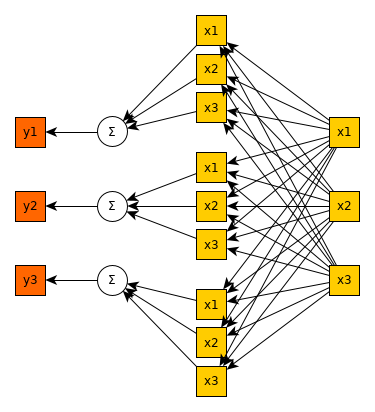
\includegraphics[scale=0.6]{quadratic-NN.png}}}
\end{equation}
but some coefficients are \textbf{redundant} because $x_i x_j = x_j x_i$.

One can eliminate redundant edges by imposing $i > j$:
\begin{equation}
\vcenter{\hbox{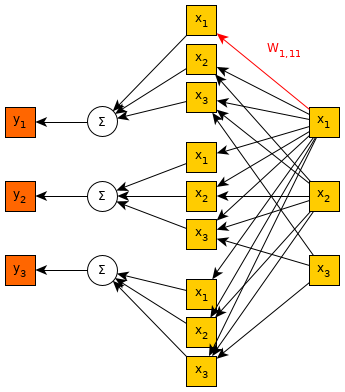
\includegraphics[scale=0.6]{quadratic-NN-2.png}}}
\end{equation}
For example, the link in red is $W_{11}^1$.  However, as we shall see below, this method creates constraints with rather complicated indices.  It appears that the first method with redundant weights is algebraically more elegant.

\subsection{Making all terms homogeneous}
\label{homogenization}

In a ``quadratic'' layer there would still be linear and constant terms.  But we can absorb them all into a single matrix $W$, making all terms homogeneous of the form: $W_{ij} x_i x_j$.

For example, the following shows part of the network with quadratic, linear, and constant terms.  The linear terms are in blue and the constant term is in green.  Notice that this block should be repeated for each output $y_1, ..., y_3$:
\begin{equation}
\vcenter{\hbox{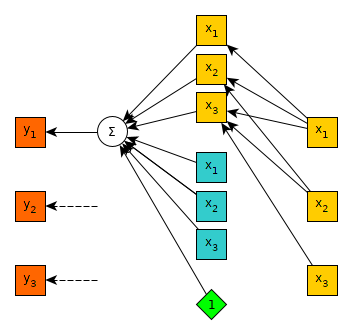
\includegraphics[scale=0.6]{quadratic-NN-3.png}}}
\end{equation}

Homogenization means adding a new input $x_4 \equiv 1$, similar to the ``bias'' term in traditional neural networks.  All the terms (quadratic, linear, constant) would be absorbed into a single matrix $W$:
\begin{equation}
\vcenter{\hbox{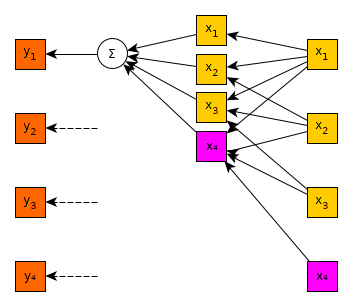
\includegraphics[scale=0.6]{quadratic-NN-4.png}}}
\end{equation}

\subsection{Linear case: $y = W x$}

\begin{equation}
\boxed{\mbox{original}} \quad y_j = \sum_i W_{ij} x_i .
\end{equation}

Equivariance implies:
\begin{eqnarray}
\boxed{\mbox{LHS}} \quad y_j ( \sigma(x_j \; x_k) x) &=& \sigma \cdot y_j = y_k \quad \boxed{\mbox{RHS}} \\
\sum_{i \neq j,k} W_{ij} x_i + W_{kj} x_j + W_{jj} x_k &=& \sum_{i \neq j,k} W_{ik} x_i + W_{jk} x_j + W_{kk} x_k . \nonumber
\end{eqnarray}

% for $(j \; k) \in \mathfrak{S}_n$.

Comparing coefficients on the LHS and RHS yields:
\begin{eqnarray}
W_{ij} &=& W_{ik} \quad \quad \forall \; j, k, (i \neq j, k) \nonumber \\
W_{kj} &=& W_{jk} \quad \quad \forall \; j, k \nonumber \\
W_{jj} &=& W_{kk} \quad \quad \forall \; j, k .
\end{eqnarray}

In other words, the matrix $W$ is of the form:
\begin{equation}
W = \alpha I + \beta 1 1^T .
\end{equation}

Python code: \\
\href{https://github.com/Cybernetic1/symmetric-NN/blob/master/sym-NN-2.py}{https://github.com/Cybernetic1/symmetric-NN/blob/master/sym-NN-2.py}

\subsection{Quadratic case: $y_k = W_k x \cdot x$ (with redundant indices)}

The general form of a ``quadratic'' vector function is:
\begin{equation}
y = (A x) \cdot x + B x + C .
\end{equation}

As described in \S\ref{homogenization}, we abosrb all weights into a single matrix, giving $(A x) \cdot x$:
\begin{equation}
\boxed{\mbox{original}} \quad y_k = \sum_j \left[ \sum_i a_{ij}^k x_i \right] x_j .
\end{equation}
Note that the matrix $A$ is ``3D'' and has $N \times N \times N$ entries.

Equivariance implies:
\begin{equation}
\boxed{\mbox{LHS}} \quad y_k ( \sigma(x_k \; x_h) \cdot x) = \sigma \cdot y_k = y_h \quad \boxed{\mbox{RHS}}
% \sum_{j \neq h,k} \sum_{i \neq h,k} a_{ij}^k x_i x_j + a_{hh}^k x_k^2 + a_{kh}^k x_h x_k + a_{hk}^k x_k x_h + a_{kk}^k x_h^2 &=& \sum_{j \neq h,k} \sum_{i \neq h,k} a_{ij}^h x_i x_j + a_{hh}^h x_h^2 + a_{kh}^h x_k x_h + a_{hk}^h x_h x_k + a_{kk}^h x_k^2 \nonumber
\end{equation}

\begin{eqnarray}
LHS &=& \sum_j \left[ \sum_{i \neq h,k} a^k_{ij} x_i + a^k_{hj} x_k + a^k_{kj} x_h \right] \sigma \cdot x_j \nonumber \\
&=& \sum_{j \neq h,k} \left[ \sum_{i \neq h,k} a^k_{ij} x_i + a^k_{hj} x_k + a^k_{kj} x_h \right] x_j
+ \left[ \sum_{i \neq h,k} a^k_{ih} x_i + a^k_{hh} x_k + a^k_{kh} x_h \right] x_k
+ \left[ \sum_{i \neq h,k} a^k_{ik} x_i + a^k_{hk} x_k + a^k_{kk} x_h \right] x_h \nonumber \\
&=& \sum_{j \neq h,k} \sum_{i \neq h,k} a^k_{ij} x_i x_j + \sum_{j \neq h,k} a^k_{hj} x_k x_j + \sum_{j \neq h,k} a^k_{kj} x_h x_j \nonumber \\
&& + \sum_{i \neq h,k} a^k_{ih} x_i x_k + a^k_{hh} x^2_k + a^k_{kh} x_h x_k \nonumber \\
&& + \sum_{i \neq h,k} a^k_{ik} x_i x_h + a^k_{hk} x_k x_h + a^k_{kk} x^2_h \nonumber \\
RHS &=& \sum_j \left[ \sum_i a_{ij}^h x_i \right] x_j \nonumber \\
&=& \sum_{j \neq h,k} \sum_{i \neq h,k} a^h_{ij} x_i x_j + \sum_{j \neq h,k} a^h_{kj} x_k x_j + \sum_{j \neq h,k} a^h_{hj} x_h x_j \nonumber \\
&& + \sum_{i \neq h,k} a^h_{ik} x_i x_k + a^h_{kk} x^2_k + a^h_{hk} x_h x_k \nonumber \\
&& + \sum_{i \neq h,k} a^h_{ih} x_i x_h + a^h_{kh} x_k x_h + a^h_{hh} x^2_h
\end{eqnarray}

Comparing coefficients on the LHS and RHS yields:
\begin{alignat}{3}
a_{ij}^h &= a_{ij}^k && \forall \; h,k, (i \neq h,k, j \neq h,k) \nonumber \\
a_{kj}^h &= a_{hj}^k && \forall \; h,k, (j \neq h,k) \nonumber \\
a_{hj}^h &= a_{kj}^k && \forall \; h,k, (j \neq h,k) \nonumber \\
a_{ik}^h &= a_{ih}^k && \forall \; h,k, (i \neq h,k) \nonumber \\
a_{ih}^h &= a_{ik}^k && \forall \; h,k, (i \neq h,k) \nonumber \\
a_{kk}^h &= a_{hh}^k && \forall \; h,k \nonumber \\
a_{hh}^h &= a_{kk}^k && \forall \; h,k \nonumber \\
a_{hk}^h + a_{kh}^h &= a_{hk}^k + a_{kh}^k \quad && \forall \; h,k .
\end{alignat}
The last constraint is not a simple equality of weights.  It arises because $x_h x_k = x_k x_h$, a consequence of the \textbf{redundancy} of the weights as explained in \S\ref{redundant-weights}.

How many distinct weights?
\begin{equation}
\begin{tabular}{c c c c}
$N = 2$ .... & 6 & / 8 & = 75\% \\
$N = 3$ .... & 9 & / 27 & = 33.3\% \\
$N = 4$ .... & 11 & / 64 & = 17/2\% \\
$N = 5$ .... & 13 & / 125 & = 10.4\% \\
$N = 6$ .... & 15 & / 216 & = 6.9\%
\end{tabular}
\end{equation}

There would be $N$ \textbf{blocks} of $N \times N$ matrices.

All diagonals consists of 2 colors, regardless of $N$ (from 2nd and 3rd equations).  This leaves $N (N - 1)$ non-diagonal entries per block.

Non-diagonal entries of different blocks are equal, if the block indices are different from the row and column indices.  Out of $N$ blocks there would be 2 different sets of non-diagonal weights.  (This comes from the 1st equation.)

The last equation causes non-diagonal weights to have a certain symmetry about the diagonal.  

Python code: \\
\href{https://github.com/Cybernetic1/symmetric-NN/blob/master/sym-NN-8.py}{https://github.com/Cybernetic1/symmetric-NN/blob/master/sym-NN-8.py}

\subsection{Quadratic case: $y_k = W_k x \cdot x$ with ordered indices}

As I said in \S\ref{redundant-weights}, ordering the weights eliminates redundancy but also leads to complicated indexing.

Recall the general form $(W x) \cdot x$:
\begin{equation}
\boxed{\mbox{original}} \quad y_k = \sum_j \left[ \sum_{i \le j} W_{ij}^k x_i \right] x_j .
\end{equation}
The matrix $W$ is ``3-dimensional'' and has $N \times N \times N$ entries.

Let $\sigma := (x_k \rightleftharpoons x_h)$, meaning \textbf{transposition} of the two elements.  Equivariance implies:
\begin{equation}
\boxed{\mbox{LHS}} \quad y_k ( \sigma \cdot x) = \sigma \cdot y_k = y_h \quad \boxed{\mbox{RHS}}
% \sum_{j \neq h,k} \sum_{i \neq h,k} W_{ij}^k x_i x_j + W_{hh}^k x_k^2 + W_{kh}^k x_h x_k + W_{hk}^k x_k x_h + W_{kk}^k x_h^2 &=& \sum_{j \neq h,k} \sum_{i \neq h,k} W_{ij}^h x_i x_j + W_{hh}^h x_h^2 + W_{kh}^h x_k x_h + W_{hk}^h x_h x_k + W_{kk}^h x_k^2 \nonumber
\end{equation}

\begin{align}
\boxed{\mbox{LHS}} &= y_k ( \sigma \cdot x ) = \sum_j \left[ \sum_{i \le j} W_{ij}^k  \; \sigma \cdot x_i \right] \sigma \cdot x_j \nonumber \\
&= \sum_j \left[ \sum_{i \le j \atop i \neq h,k} W^k_{ij} x_i + \underbracket[1pt]{W^k_{hj} x_k}_{\text{if } h \le j} + \underbracket[1pt]{W^k_{kj} x_h}_{\text{if } k \le j} \right] \sigma \cdot x_j \quad \quad \boxed{\text{applied } \sigma \cdot x_i} \nonumber \\
% 
&= \sum_{j \neq h,k} \left[ \sum_{i \le j \atop i \neq h,k} W^k_{ij} x_i + \underbracket[1pt]{W^k_{hj} x_k}_{\text{if } h \le j} + \underbracket[1pt]{W^k_{kj} x_h}_{\text{if } k \le j} \right] x_j 
	\quad \quad \quad \boxed{\text{applied } \sigma \cdot x_j} \nonumber \\
	& \quad \quad + \left[ \sum_{i < h \atop i \neq k} W^k_{ih} x_i + W^k_{hh} x_k + \underbracket[1pt]{W^k_{kh} x_h}_{\text{if } k \le h} \right] x_k
	+ \left[ \sum_{i < k \atop i \neq h} W^k_{ik} x_i + \underbracket[1pt]{W^k_{hk} x_k}_{\text{if } h \le k} + W^k_{kk} x_h \right] x_h \nonumber \\
% 
&= \sum_{j \neq h,k} \sum_{i \le j \atop i \neq h,k} W^k_{ij} x_i x_j + {\color{olive}\sum_{j > h} W^k_{hj} x_k x_j} + {\color{cyan}\sum_{j > k} W^k_{kj} x_h x_j} \nonumber \\
& \quad \quad + {\color{blue}\sum_{i < h \atop i \neq k} W^k_{ih} x_i x_k} + W^k_{hh} x_k^2 + {\color{green}  \underbracket[1pt]{W^k_{kh} x_h x_k}_{\text{if } k \le h}} \nonumber \\
& \quad \quad + {\color{red}\sum_{i < k \atop i \neq h} W^k_{ik} x_i x_h} + {\color{violet} \underbracket[1pt]{W^k_{hk} x_k x_h}_{\text{if } h \le k} } + W^k_{kk} x_h^2 \nonumber \\
% 
% ============================================================================================
% 
\boxed{\mbox{RHS}} &= \sum_j \left[ \sum_{i \le j} W_{ij}^h x_i \right] x_j \nonumber \\
% 
&= \sum_j \left[ \sum_{i \le j \atop i \neq h,k} W^h_{ij} x_i + \underbracket[1pt]{W^h_{hj} x_h}_{\text{if } h \le j} + \underbracket[1pt]{W^h_{kj} x_k}_{\text{if } k \le j} \right] x_j \nonumber \\
% 
&= \sum_{j \neq h,k} \left[ \sum_{i \le j \atop i \neq h,k} W^h_{ij} x_i + \underbracket[1pt]{W^h_{hj} x_h}_{\text{if } h \le j} + \underbracket[1pt]{W^h_{kj} x_k}_{\text{if } k \le j} \right] x_j \nonumber \\
& \quad \quad + \left[ \sum_{i < h \atop i \neq k} W^h_{ih} x_i + W^h_{hh} x_h + \underbracket[1pt]{W^h_{kh} x_k}_{\text{if } k \le h} \right] x_h
+ \left[ \sum_{i < k \atop i \neq h} W^h_{ik} x_i + \underbracket[1pt]{W^h_{hk} x_h}_{\text{if } h \le k} + W^h_{kk} x_k \right] x_k \nonumber \\
% 
&= \sum_{j \neq h,k} \sum_{i \le j \atop i \neq h,k} W^h_{ij} x_i x_j + {\color{cyan}\sum_{j > h} W^h_{hj} x_h x_j} + {\color{olive}\sum_{j > k} W^h_{kj} x_k x_j} \nonumber \\
& + {\color{red}\sum_{i < h \atop i \neq k} W^h_{ih} x_i x_h} + W^h_{hh} x_h^2 + {\color{green} \underbracket[1pt]{W^h_{kh} x_k x_h}_{\text{if } k \le h}} \nonumber \\
& + {\color{blue}\sum_{i < k \atop i \neq h} W^h_{ik} x_i x_k} + {\color{violet}\underbracket[1pt]{W^h_{hk} x_h x_k}_ {\text{if } h \le k} } + W^h_{kk} x_k^2
\label{eqn:colorful}
\end{align}

Comparing coefficients yields the following equations (except for the ``colorful'' ones):
\begin{alignat}{3}
W_{ij}^h &= W_{ij}^k \quad \quad && \forall \; i,j,h,k. \; i,j \neq h,k; \; i \le j \nonumber \\
%{\color{cyan}W_{hj}^h} &= {\color{cyan}W_{kj}^k} && \forall \; h,k. \; j > \max(h,k) \nonumber \\
%{\color{olive}W_{kj}^h} &= {\color{olive}W_{hj}^k} && \forall \; h,k. \; j > \max(h,k) \nonumber \\
%{\color{cyan}W_{hj}^h} &= {\color{olive}W_{hj}^k} = 0 \quad && \forall \; h,k. \; h < j \le k \nonumber \\
%{\color{olive}W_{kj}^h} &= {\color{cyan}W_{kj}^k} = 0 \quad && \forall \; h,k. \; k < j \le h \nonumber \\
%{\color{red}W_{ih}^h} &= {\color{red}W_{ik}^k} && \forall \; h,k. \; i \le k; \; i \neq h \nonumber \\
%{\color{blue}W_{ik}^h} &= {\color{blue}W_{ih}^k} && \forall \; h,k. \; i \le h; \; i \neq k \nonumber \\
%{\color{red}W_{kh}^h} &= {\color{red}W_{kh}^k} && \forall \; h,k. \; k \le h \nonumber \\
%{\color{blue}W_{hk}^h} &= {\color{blue}W_{hk}^k} && \forall \; h,k. \; h \le k \nonumber \\
\boxed{\mbox{``Black'' equations}} \quad \quad W_{hh}^k &= W_{kk}^h && \forall \; h,k. \nonumber \\
W_{kk}^k &= W_{hh}^h && \forall \; h,k.
\label{eqn:black-ones}
\end{alignat}

The colored terms lead to these constraints:
\begin{alignat}{3}
\mbox{cases} & && h < k: \nonumber \\
\mbox{{\color{cyan}cyan} = {\color{cyan}cyan}} \quad \quad W^k_{ki} &= W^h_{hi} \quad \quad && \forall \; i,h,k. \; i > k \nonumber \\
\mbox{{\color{olive}olive} = {\color{olive}olive}} \quad \quad W^k_{hi} &= W^h_{ki} \quad \quad && \forall \; i,h,k. \; i > k \nonumber \\
\mbox{{\color{red}red} = {\color{red}red}} \quad \quad W^k_{ik} &= W^h_{ih} \quad \quad && \forall \; i,h,k. \; i < h \nonumber \\
\mbox{{\color{blue}blue} = {\color{blue}blue}} \quad \quad W^k_{ih} &= W^h_{ik} \quad \quad && \forall \; i,h,k. \; i < h \nonumber \\
\mbox{{\color{red}red} = {\color{cyan}cyan}} \quad \quad W^k_{ik} &= W^h_{hi} \quad \quad && \forall \; i,h,k. \; h < i < k \nonumber \\
\mbox{{\color{olive}olive} = {\color{blue}blue}} \quad \quad W^k_{hi} &= W^h_{ik} \quad \quad && \forall \; i,h,k. \; h < i < k \nonumber \\
\mbox{{\color{violet}violet} = {\color{violet}violet}} \quad \quad W^h_{hk} &= W^k_{hk} \quad \quad && \forall \; h,k. \; h < k \nonumber \\
%
\mbox{cases} & && k < h: \nonumber \\
\mbox{{\color{cyan}cyan} = {\color{cyan}cyan}} \quad \quad W^k_{ki} &= W^h_{hi} \quad \quad && \forall \; i,h,k. \; i > h \nonumber \\
\mbox{{\color{olive}olive} = {\color{olive}olive}} \quad \quad W^k_{hi} &= W^h_{ki} \quad \quad && \forall \; i,h,k. \; i > h \nonumber \\
\mbox{{\color{red}red} = {\color{red}red}} \quad \quad W^k_{ik} &= W^h_{ih} \quad \quad && \forall \; i,h,k. \; i < k \nonumber \\
\mbox{{\color{blue}blue} = {\color{blue}blue}} \quad \quad W^k_{ih} &= W^h_{ik} \quad \quad && \forall \; i,h,k. \; i < k \nonumber \\
\mbox{{\color{cyan}cyan} = {\color{red}red}} \quad \quad W^k_{ki} &= W^h_{ih} \quad \quad && \forall \; i,h,k. \; k < i < h \nonumber \\
\mbox{{\color{blue}blue} = {\color{olive}olive}} \quad \quad W^k_{ih} &= W^h_{ki} \quad \quad && \forall \; i,h,k. \; k < i < h \nonumber \\
\mbox{{\color{green}green} = {\color{green}green}} \quad \quad W^h_{kh} &= W^k_{kh} \quad \quad && \forall \; h,k. \; k < h 
\end{alignat}
where notations such as ``{\color{red}red} = {\color{red}red}'' mean that the term of the first color on the LHS is compared to the term of the second color on the RHS.

The indexing situation can get a bit complicated.  For example, the following diagram shows the situation of $k > h$ with the index $j$:
\begin{equation}
\vcenter{\hbox{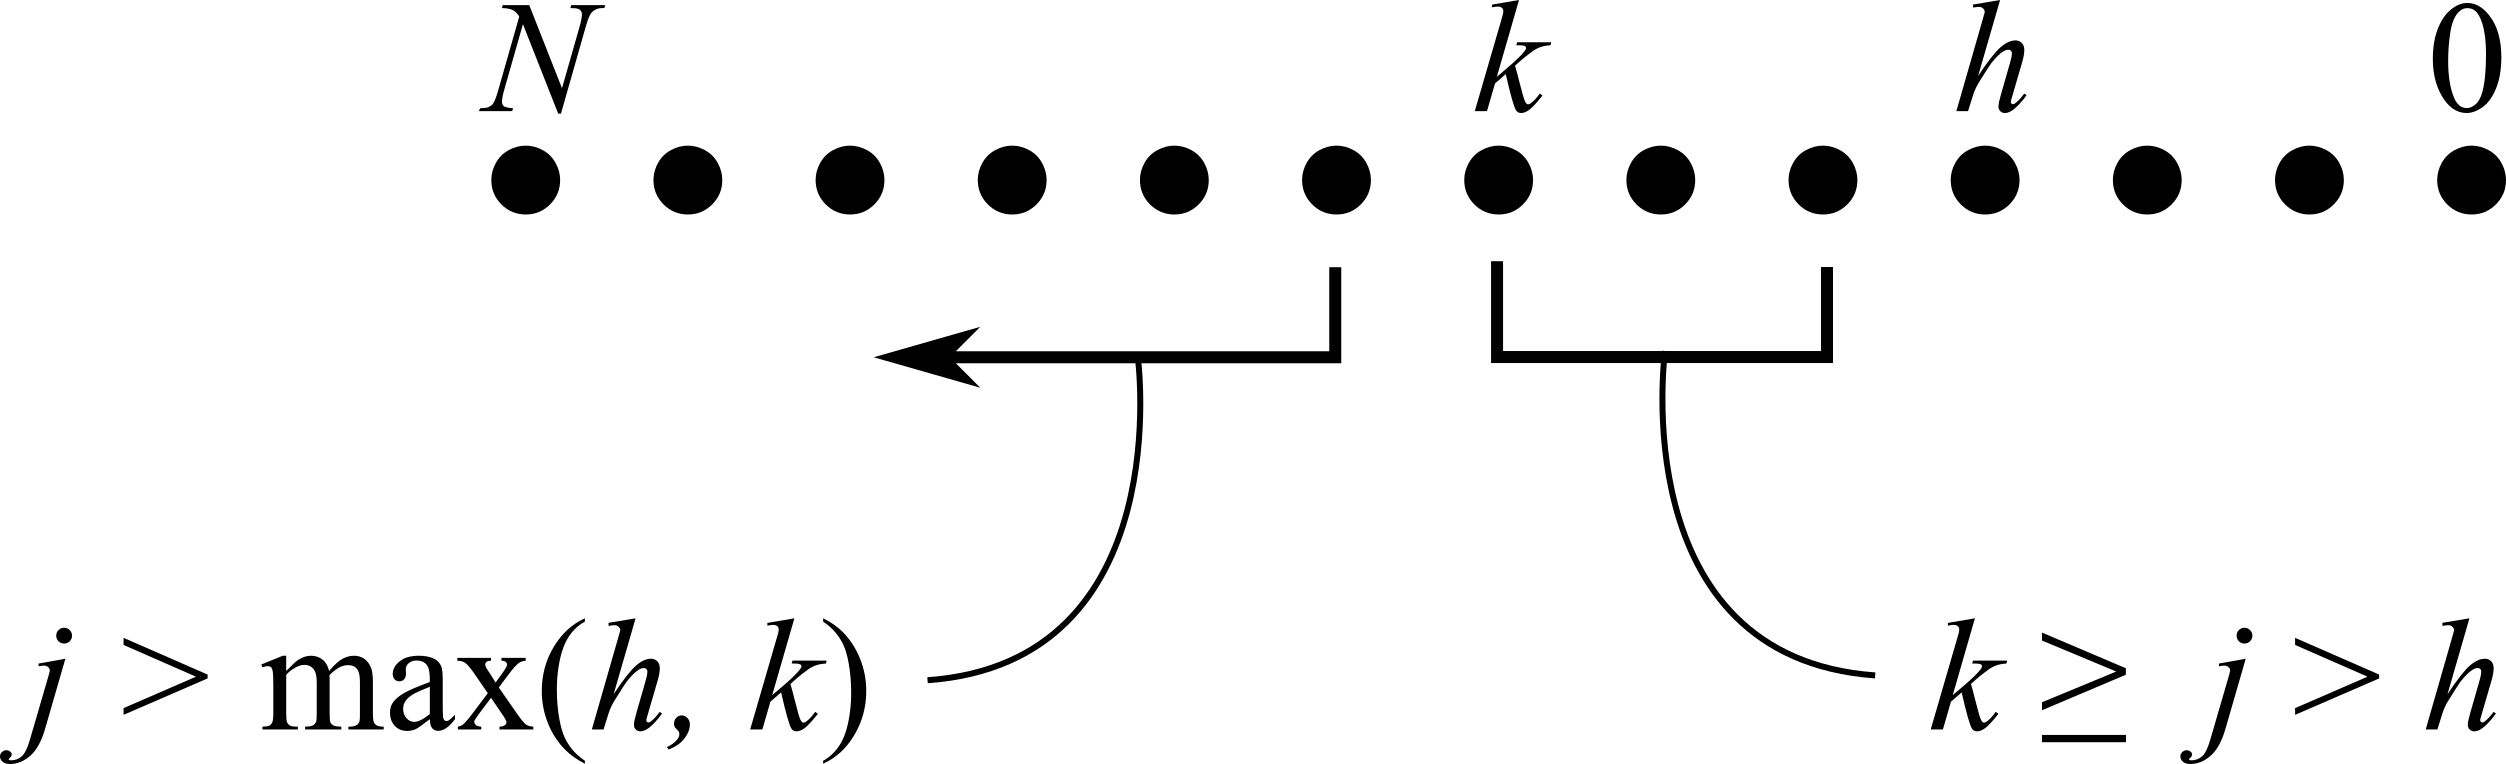
\includegraphics[scale=0.6]{index-j-diagram.png}}}
\end{equation}

The following diagram shows the indexing situation for the colored terms in equation (\ref{eqn:colorful}).  The LHS and RHS of this equation has terms with different indexings conditions:
\begin{equation}
\vcenter{\hbox{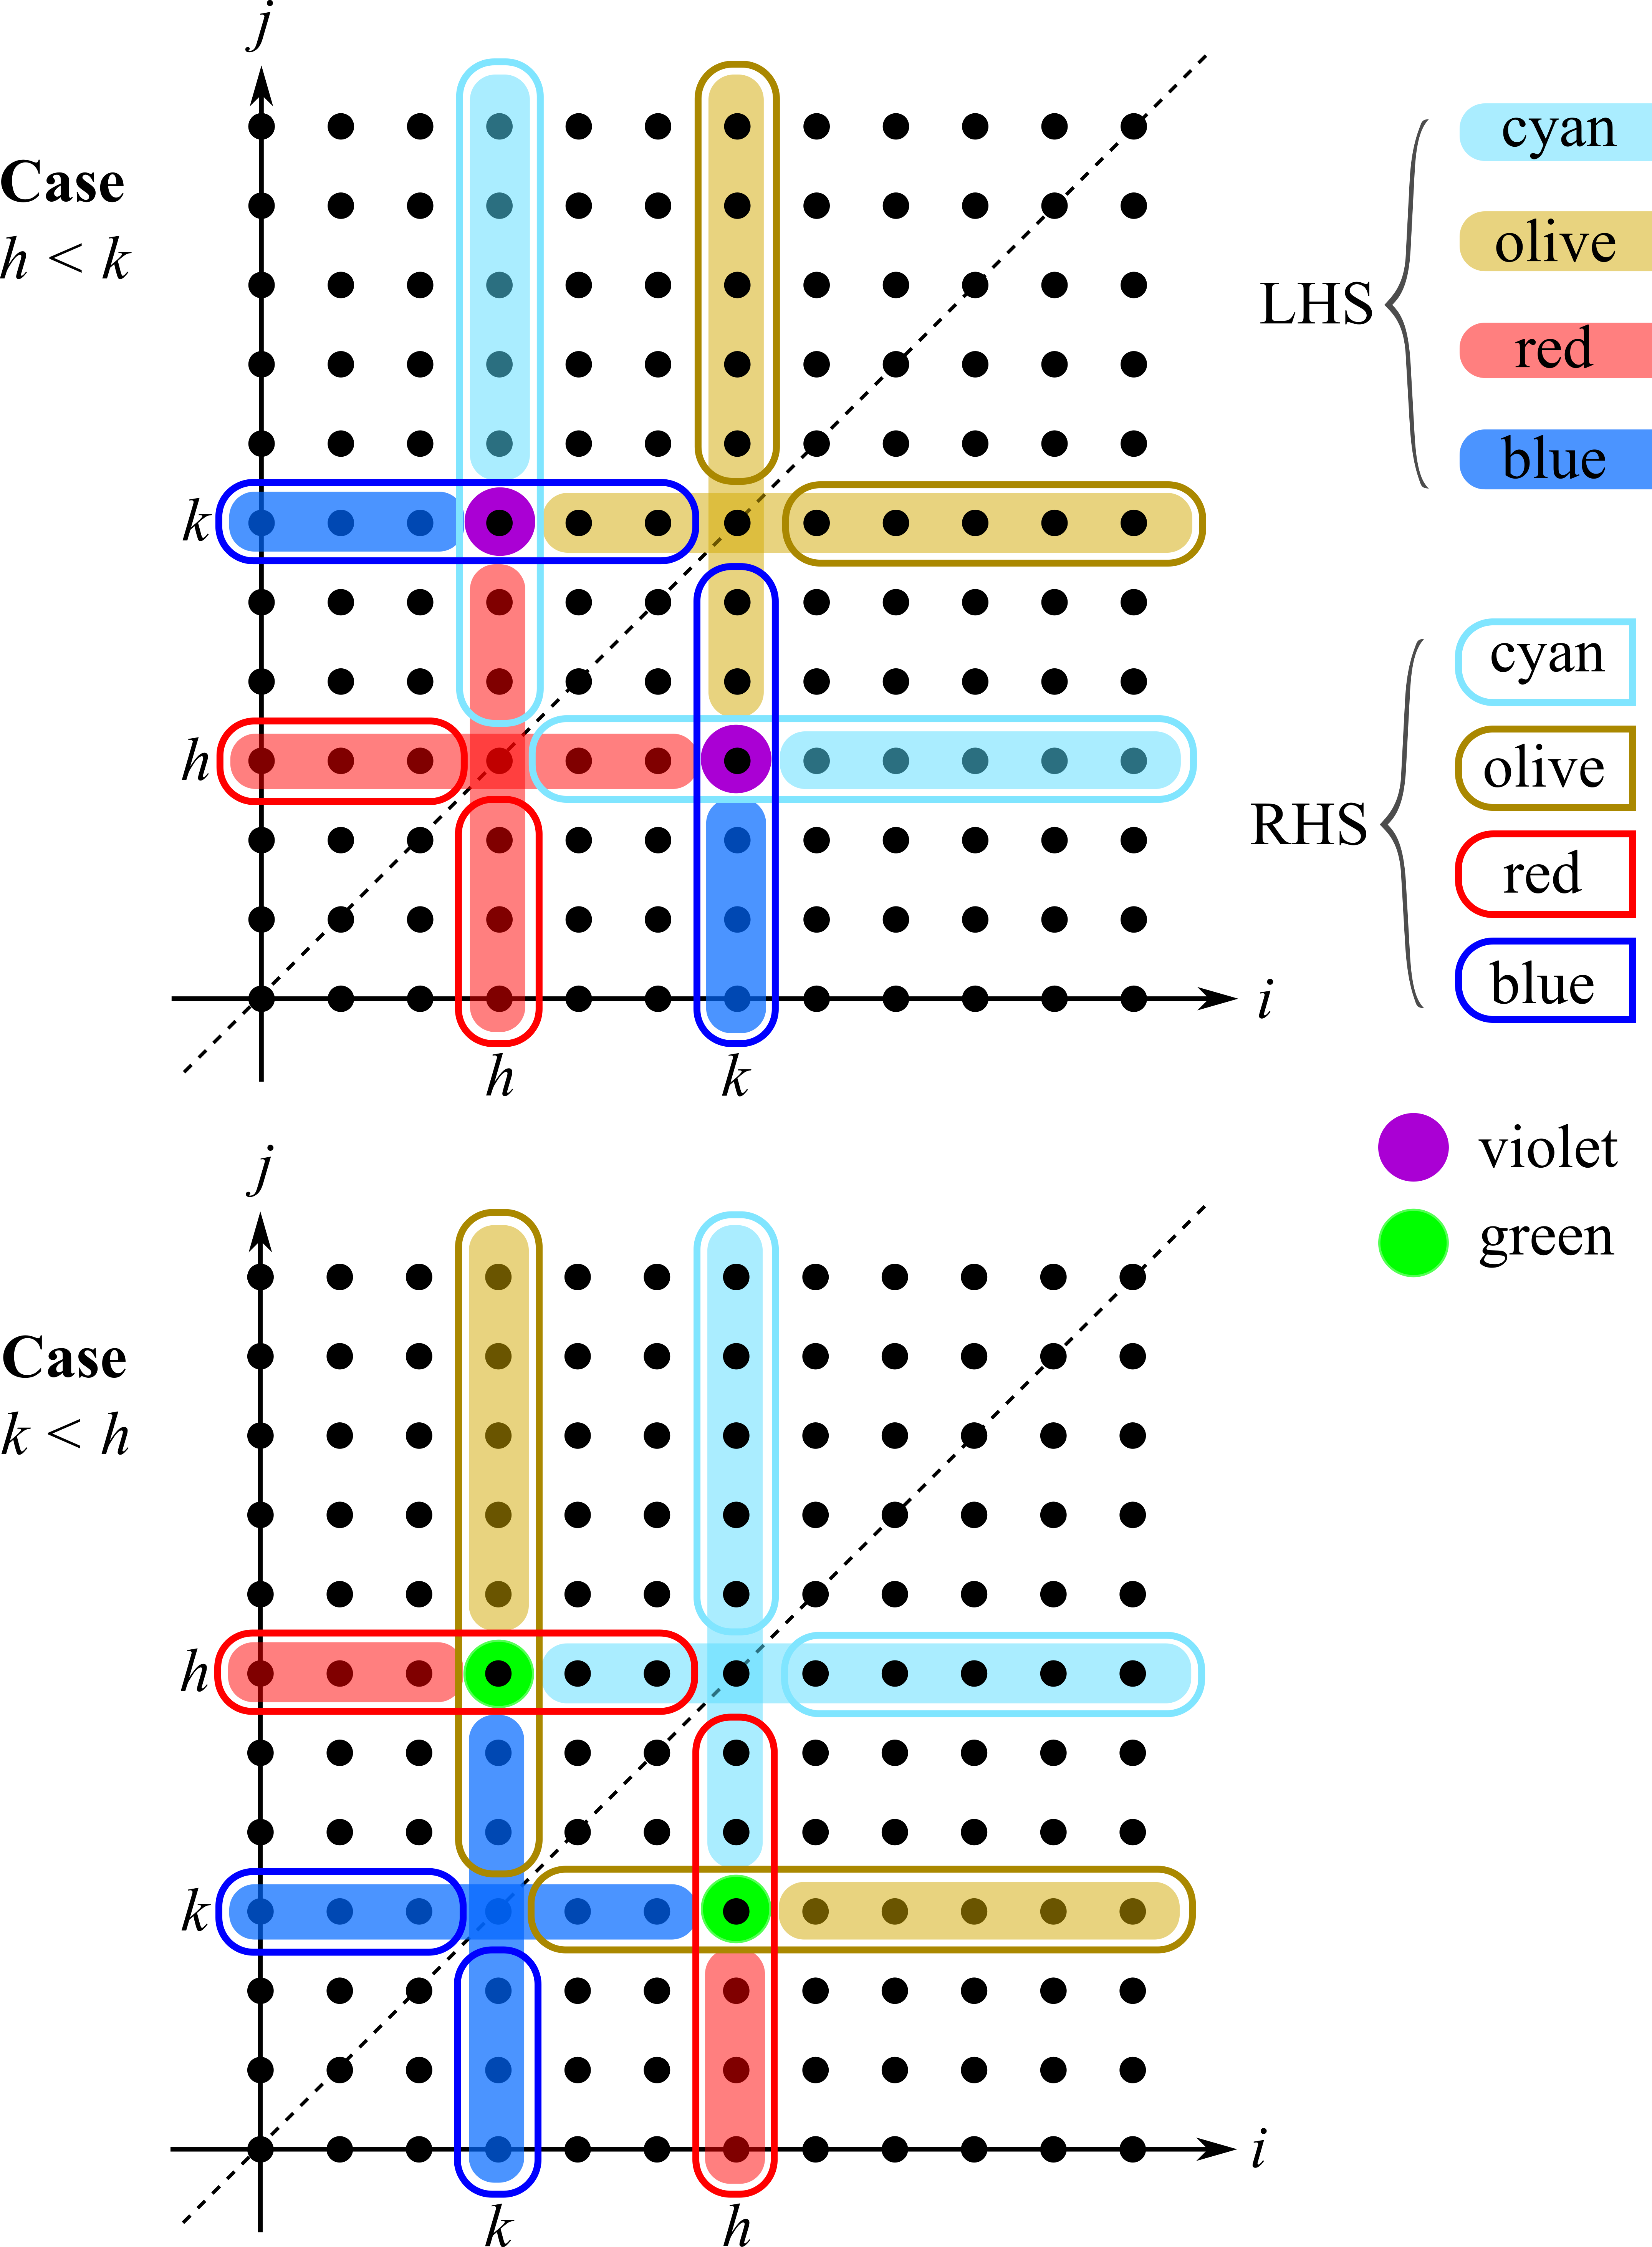
\includegraphics[scale=0.6]{index-grid-2D.png}}}
\end{equation}

It is not easy to see how many distinct weights are permitted by the constraints.  Surprisingly, Python experiments suggest that the number of distinct weights $\equiv 4$ for all $N$ (except for $N = 1, 2$ which has only 1 and 3 weights).

For example, the number of monomials in 3 variables and of degree $\le 8$ is:
\begin{eqnarray}
{10\choose8} + {9\choose7} + {8\choose6} + .... + {4\choose2} + {3\choose1} + {3\choose0} \nonumber \\
= 45 + 36 + 28 + 21 + 15 + 10 + 6 + 3 + 1 = 165
\end{eqnarray}

Python code: \\
\href{https://github.com/Cybernetic1/symmetric-NN/blob/master/sym-NN-9.py}{https://github.com/Cybernetic1/symmetric-NN/blob/master/sym-NN-9.py}

\subsection{Programmatic way to find invariant constraints on weights}

What we do here is to use a Python program to algebraically (using \textbf{symbolic} algebra) compute the invariant constraints.  This can be achieved by over-loading Python operators (such as $+, -, *$) to handle symbolic polynomials.

Python code: \\
\href{https://github.com/Cybernetic1/symmetric-NN/blob/master/poly-algebra-2.py}{https://github.com/Cybernetic1/symmetric-NN/blob/master/poly-algebra-2.py}

This is an example output (polynomial terms are ungrouped):
\begin{equation}
\vcenter{\hbox{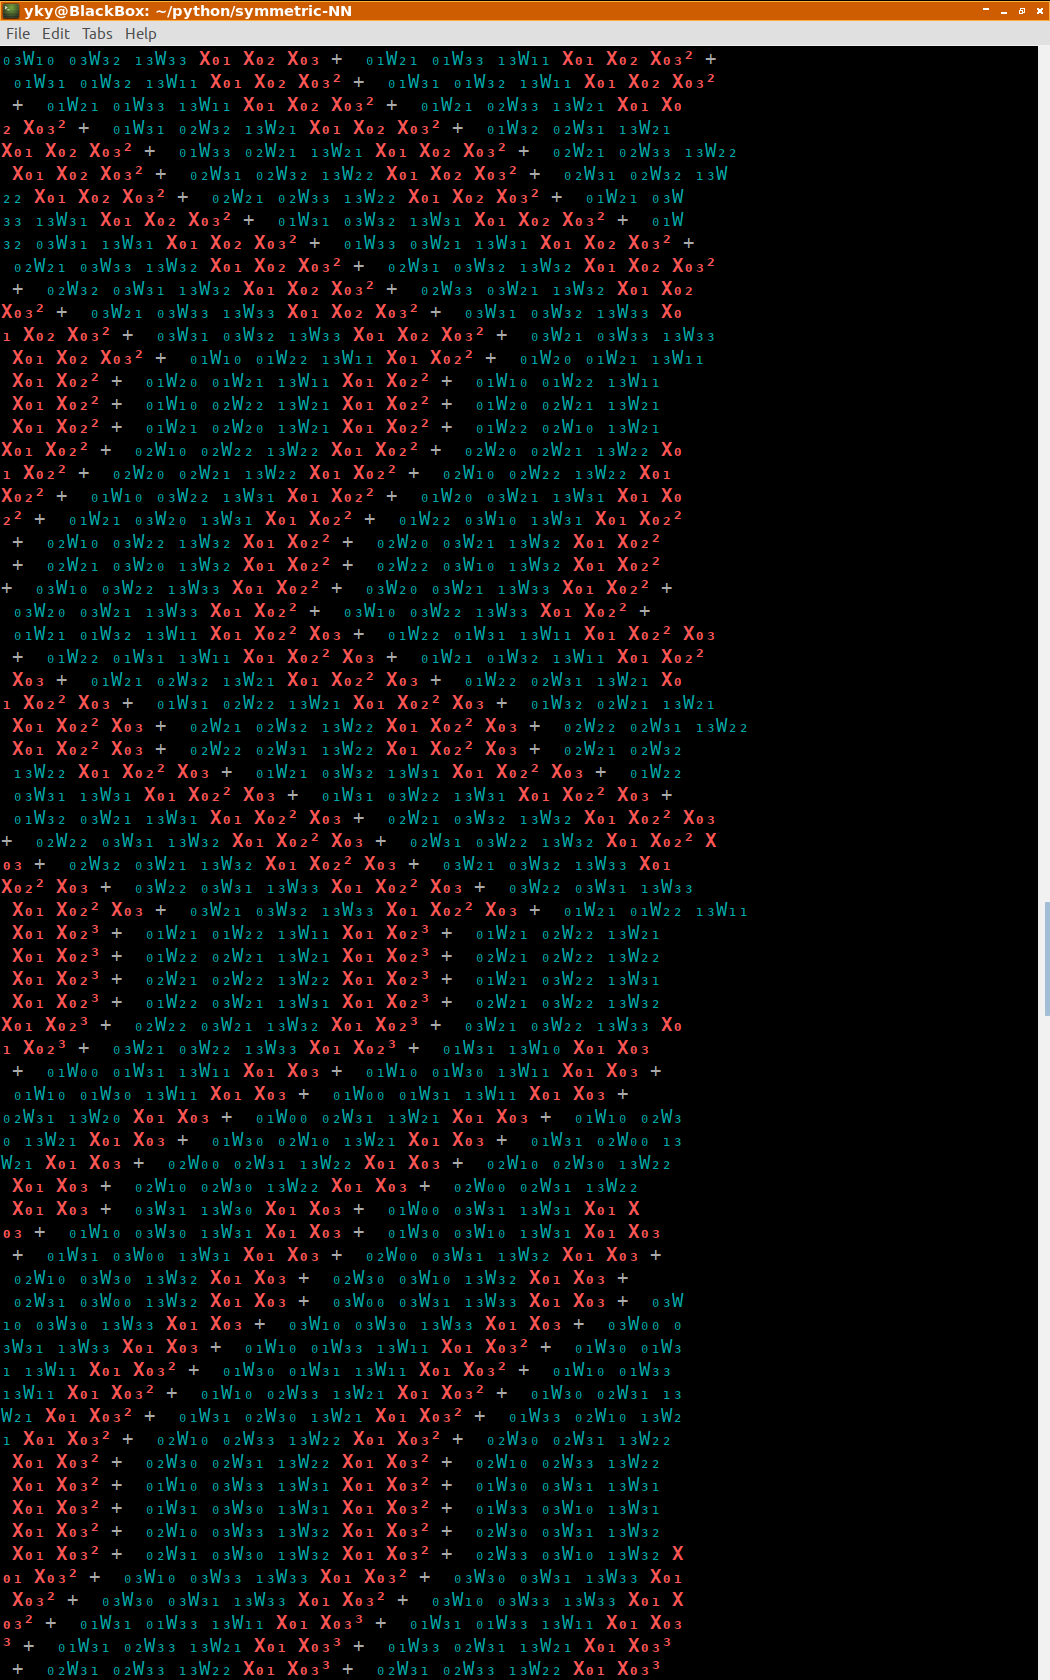
\includegraphics[scale=0.5,trim=0 400 0 0,clip]{example-ungrouped-polynomial.png}}}
\end{equation}

This is another example output (polynomial terms are grouped):
\begin{equation}
\vcenter{\hbox{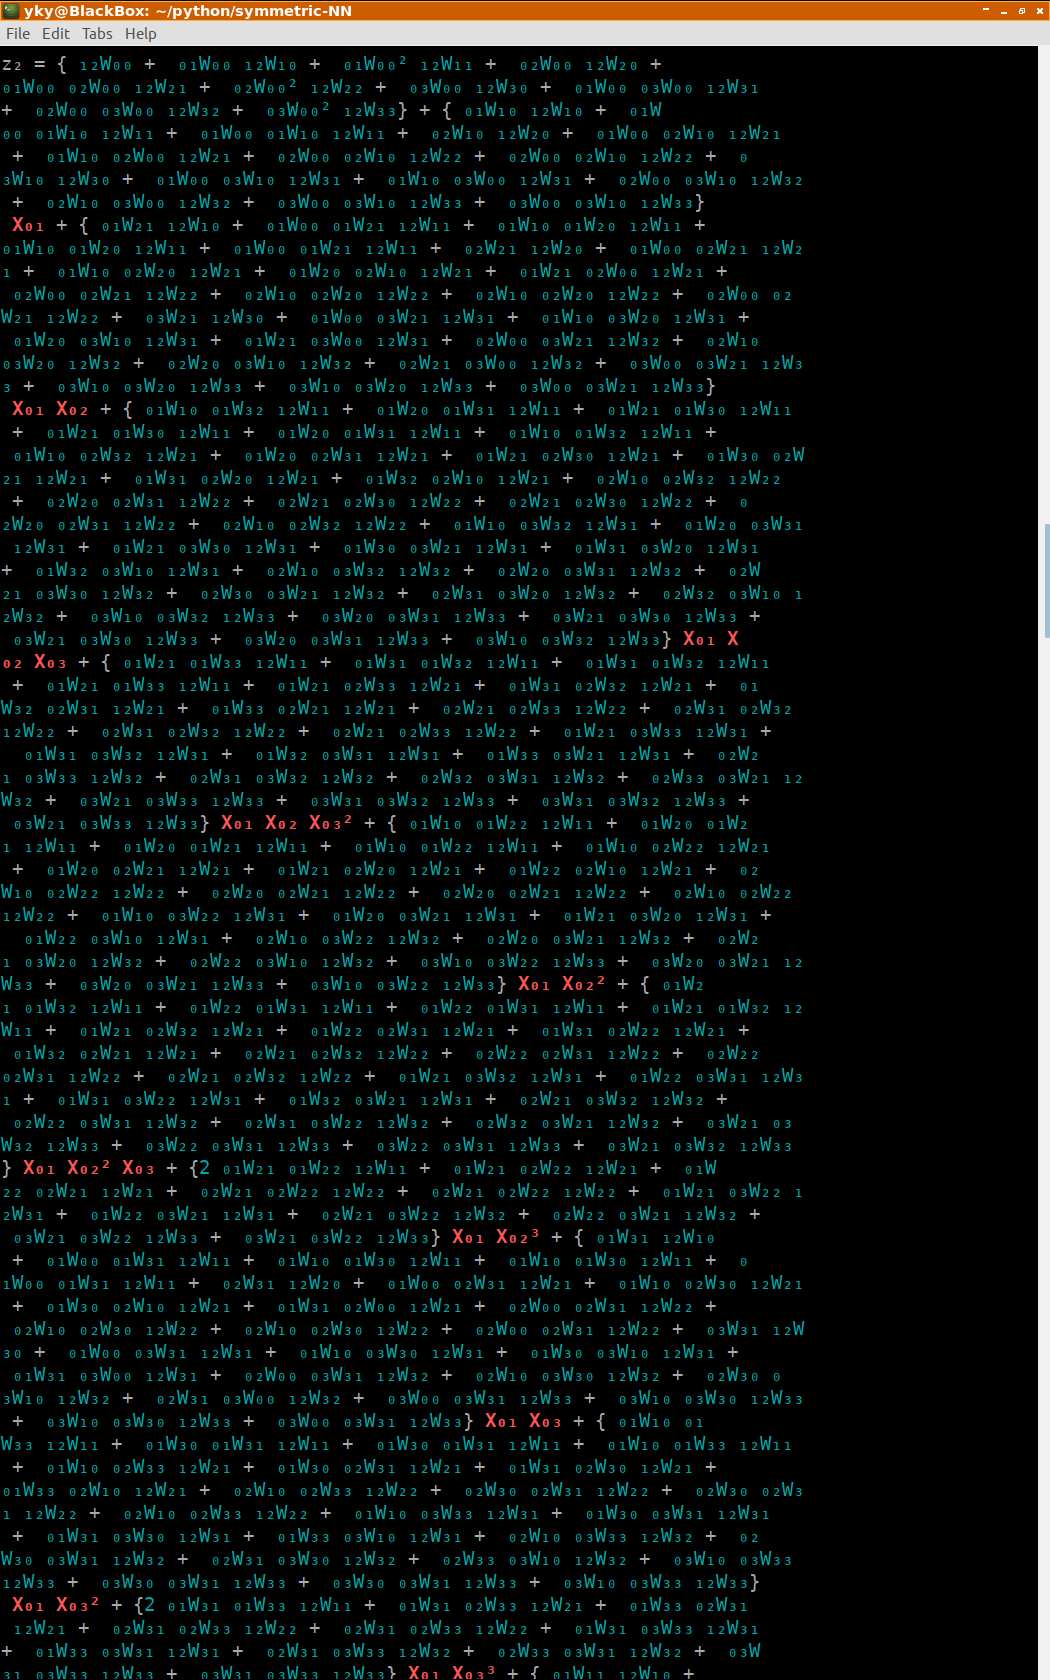
\includegraphics[scale=0.5]{z_2-polynomial.png}}}
\end{equation}

Define a scheme to index all the weights in the multi-layer NN: $W_{ij}^{k \ell}$.  Then the entire NN function can be expanded as a polynomial with coefficients from $W$.

For one quadratic layer, there would be a total of $\displaystyle n \left( n^2 - \frac{n (n - 1)}{2} \right) = \frac{n^2 (n + 1)}{2}$ terms.  The coefficients for each term would be composed out of $W_{ij}^{k \ell}$.  Permuting the input would require coefficients of \textbf{like} terms to be equal.  We should try all pairwise permutations of $n$ inputs, of which there are $n (n - 1) / 2$.

On the second layer, the output would be composed of sums and products of polynomials with second-layer weights.  Thus the new coefficients would be \textbf{polynomials} in multi-layer weights.  Invariance or equivariance requires that we compare coefficients of like terms, thus yielding \textbf{equalities with polynomials} on both sides.  Such conditions seems much more complex than the single-layer conditions for equivariance.

This means that the weights would be in an \textbf{algebraic variety} of reduced dimension.  Our objective is to update / learn the weights \textbf{within} this variety.  

\subsection{Quadratic, 2-layer case}

In the last section we have \textbf{equivariant} layers composed together to form a neural network.  Now we relax the constraints so that the multi-layer network is free to have any weights except that the output must be \textbf{equivariant} or \textbf{invariant}.

\subsection{Back-propagation algorithm for constrained weights}

作者:zighouse

链接:\url{https://www.zhihu.com/question/327765164/answer/704606353}

{\footnotesize 来源:知乎 / 著作权归作者所有。商业转载请联系作者获得授权,非商业转载请注明出处。}

神经网络是对一类内部结构固定的非线性函数的俗称,这类函数是输出关于输入以及隐含内部状态的函数,输出与输入呈现非线性特性。当一份输出只与一份输入有关时,常用卷积神经网络来实现。当一份输出与一个相继表达的输入序列相关时,可以用回归神经网络来实现。一般地,神经网络可以技术性地分解成神经元的复合,这里的神经元是在这个神经网络中的一种最基本的非线性函数的俗称,管理着属于它的内部状态,并基于这些内部状态在神经网络中负责着分配到它的非线性处理。每多一重基本非线性函数的复合,则多一层神经元。如果在某一重复合中出现了两类或者更多类基本非线性函数项的合并,则出现了分支。

神经网络的权值是分解到具体神经元管理的一种内部状态。用反向传播方法来更新神经网络的权值是基于这样一个基本的假设:在一个确定的输入(或者输入序列)并产生当前输出的这个点(权值构成的线性空间中的点)上,输出在这个点上是连续的。即权值点的连续微小变化会导致输出点相应的连续微小变化。这样,当我们希望调节当前权值以使此输出向特定点靠拢时,就得出了基于权值空间中错误/误差/惩罚的梯度的反向传播算法。

如果想在某个神经网络中的两个权值间建立一种约束关系,这两个权值自然就不再相互独立,可以通过考查整个权值构成的线性空间,秩会变小。约束条件只要不改变连续假设,仍然可以求出带约束条件下的梯度。如果改变了连续假设,则意味着非线性分解不恰当,需要重新分解神经网络的基本结构。

\subsubsection{Quadratic NN setup}

Traditional neural network:
\begin{eqnarray}
\boxed{neuron} \quad & y = & \sigmoid \vect{w} \cdot \vect{x} \nonumber \\
\boxed{layer} \quad & y = & \sigmoid W \vect{x} \nonumber \\
\boxed{network} \quad & y = & \sigmoid W \circ \sigmoid W \; .... \; \vect{x} 
\end{eqnarray}

Quadratic neural network:
\begin{eqnarray}
\boxed{neuron} \quad & y = & \langle W \vect{x}, \vect{x} \rangle \nonumber \\
\boxed{layer} \quad & y = & \langle W \vect{x}, \vect{x} \rangle \nonumber \\
\boxed{network} \quad & y = & \langle W \vect{x}, \vect{x} \rangle \circ \langle W \vect{x}, \vect{x} \rangle \; .... \; \vect{x} 
\end{eqnarray}

Traditionally, each neuron $k$ with output $o_k$ is defined as:
\begin{equation}
o_k = \sigmoid ({\text{net}}_k) = \sigmoid \left(\sum _{j=1}^{n} w_{jk} o_j \right) .
\end{equation}

This is replaced by our new neuron:
\begin{equation}
\boxed{\mbox{next layer}} \quad
o_k = {\text{net}}_k = \sum_j \sum_i W_{ij}^k o_i o_j
\quad \boxed{\mbox{current layer}}
\end{equation}
where the 2 summations can be \textbf{interchanged}.

\subsubsection{Classical back-prop algorithm}

What follows is just a re-working of traditional back-propagation.  For ease of comparison, let's recall the classic derivation of the back-prop algorithm (from Wikipedia):

The weight update rule is:
\begin{equation}
\Delta W_{ij} = - \eta \frac{\partial E}{\partial W_{ij}} = - \eta o_i \delta_j
\end{equation}
where $\delta_j$ is the so-called ``local gradient''.  $o_i$ is the $i$-th output, $\eta$ is the learning rate.

The gradient is:
\begin{equation}
	\label{eqn:back-prop-chain-rule}
\frac{\partial E}{\partial W_{ij}}
= \frac{\partial E}{\partial o_j} \frac{\partial o_j}{\partial W_{ij}}
= {\color{red} \frac{\partial E}{\partial o_j}} \cdot
  {\color{olive} \frac{\partial o_j}{\partial \mathrm{net}_j}} \cdot
  {\color{cyan} \frac{\partial \mathrm{net}_j}{\partial W_{ij}}} .
\end{equation}
In the last factor on the RHS, only one term in $\mathrm{net}_j$ depends on $W_{ij}$, so:
\begin{equation}
{\color{cyan} \frac{\partial \mathrm{net}_j}{\partial W_{ij}}}
= \frac{\partial}{\partial W_{ij}} \left( \sum_k W_{kj} o_k \right)
= \frac{\partial}{\partial W_{ij}} W_{ij} o_i = o_i .
\end{equation}
The middle factor on the RHS is the partial derivative of the activation function:
\begin{equation}
{\color{olive} \frac{\partial o_j}{\partial \mathrm{net}_j}}
= \frac{\partial \sigmoid(\mathrm{net}_j)}{\partial \mathrm{net}_j} .
\end{equation}
The first factor is easy to evaluate if the neuron is in the output layer:
\begin{equation}
{\color{red} \frac{\partial E}{\partial o_j}}
= \frac{\partial}{\partial o_j} \frac{1}{2} (o^* - o_j)^2 = o_j - o^* = \epsilon
\end{equation}
where $\epsilon$ is the error.

Otherwise, assume $\mathcal{C}$ is the set of all child neurons \textbf{receiving} input from neuron $j$, one gets a \textbf{recursive} expression for the derivative:
\begin{equation}
{\color{red} \frac{\partial E}{\partial o_j}}
= \sum_{c \in \mathcal{C}} \left( \frac{\partial E}{\partial \mathrm{net}_c} \frac{\partial \mathrm{net}_c}{\partial o_j} \right)
= \sum_{c \in \mathcal{C}} \left( \frac{\partial E}{\partial o_c} \frac{\partial o_c}{\partial \mathrm{net}_c} \frac{\partial \mathrm{net}_c}{\partial o_j} \right)
= \sum_{c \in \mathcal{C}} \left( \frac{\partial E}{\partial o_c} \frac{\partial o_c}{\partial \mathrm{net}_c} W_{jc} \right)
\end{equation}

So we get the \boxed{\mbox{classic back-prop algorithm}}\ :
\begin{eqnarray}
\frac{\partial E}{\partial W_{i j}} &=&  \delta_j \cdot {\color{cyan} o_i} \nonumber \\
\delta_j &=& {\color{red} \frac{\partial E}{\partial o_j}} \cdot {\color{olive} \frac{\partial o_j}{\partial \mathrm{net}_j}} =
\begin{cases}
\displaystyle
{\color{red} \frac{\partial E}{\partial o_j}} \cdot {\color{olive} \frac{\partial \sigmoid(\mathrm{net}_j)}{\partial \mathrm{net}_j}} & \text{if $j$ = output neuron} \\
\displaystyle
{\color{red} \sum_c W_{j c} \cdot \delta_c} \cdot {\color{olive} \frac{\partial \sigmoid(\mathrm{net}_j)}{\partial \mathrm{net}_j}} &  \text{if $j$ = inner neuron} 
\end{cases}
\end{eqnarray}

\subsubsection{Quadratic back-prop algorithm}

Applying the chain rule as in (\ref{eqn:back-prop-chain-rule}):
\begin{equation}
\frac{\partial E}{\partial W_{ij}^k}
= {\color{red} \frac{\partial E}{\partial o_k}} \cdot {\color{cyan} \frac{\partial o_k}{\partial W_{ij}^k}} .
\end{equation}
Notice that we don't use an activation function, so the {\color{olive}olive} factor disappears.

For the RHS's second factor, only one term in the sum depends on $W_{ij}^k$, so:
\begin{equation}
	\label{eqn:do-k-dW}
{\color{cyan} \frac{\partial o_k}{\partial W_{ij}^k}}
= \frac{\partial }{\partial W_{ij}^k} \left( \sum_{i'} \sum_{j'} W_{i' j'}^k o_{i'} o_{j'} \right)
= \frac{\partial }{\partial W_{ij}^k} W_{ij}^k o_i o_j = o_i o_j .
\end{equation}

If $k$ is an inner neuron, let $\mathcal{C} = \{ u, v, \dots , w \}$ be the \textbf{next layer} of neurons receiving input from neuron $k$.  Consider $E$ as a function with the inputs being all neurons in $\mathcal{C}$:
\begin{eqnarray}
\frac{\partial E(o_k)}{\partial o_k}
&=& \frac{\partial E(o_u, o_v, \dots, o_w)}{\partial o_k} \nonumber \\
\boxed{\mbox{next layer}} \quad
	o_c &=& \sum_j \sum_i W_{ij}^c o_i o_j
\quad \boxed{\mbox{current layer}} .
\end{eqnarray}
Then the \textbf{recursive} expression for the derivative is obtained:
\begin{equation}
	\label{eqn:dE-do-k}
{\color{red} \frac{\partial E}{\partial o_k}}
= \sum_{c \in \mathcal{C}} \left( \frac{\partial E}{\partial o_c} \frac{\partial o_c}{\partial o_k} \right)
= \sum_{c \in \mathcal{C}} \left( \frac{\partial E}{\partial o_c} \sum_j W_{kj}^c o_j \right)
\end{equation}

Substituting, we obtain the algorithm:
\begin{eqnarray}
\boxed{\mbox{quadratic back-prop}} \quad \quad
\frac{\partial E}{\partial W_{ij}^k}
&=& \frac{\partial E}{\partial o_k} \frac{\partial o_k}{\partial W_{ij}^k}
= \frac{\partial E}{\partial o_k} o_i o_j := {\color{red} \delta_k} \cdot {\color{cyan} o_i o_j} \nonumber \\ 
{\color{red} \delta_k} &:=& {\color{red} \sum_{c \in \mathcal{C}} \left( \delta_c \sum_j W_{kj}^c o_j \right)}
\end{eqnarray}

\subsubsection{Shared weights}

For the single-layer (stacked) case, it is good to know that all the weight-sharing occurs \textbf{within} each layer, never across layers.

The coefficient of $x_i x_j$ is $W_{i j}$, for the $y_k$ component.  For each weight $W_{ij}^k$ we need to calculate the gradient $\displaystyle \frac{\partial E}{\partial W_{ij}^k}$, but the weights are in equivalence classes.

Say if the following 2 weights are shared:
\begin{equation}
W_0 := W_{i j} \equiv W_{i' j'}
\end{equation}
Then the network:
\begin{equation}
y = \sum \sum W_{ij} x_i x_j
\end{equation}
would contain the shared components:
\begin{equation}
W_0 ( x_i x_j + x_{i'} x_{j'} ) + \mbox{other terms ...}
\end{equation}

\subsubsection{Equality constraints}

For simple \textbf{equality} of weights, the weights should be collected together.  (\ref{eqn:do-k-dW}) should simply be $\sum o_i o_j$ for the equivated weights.

\subsubsection{Additive constraints}

The most tricky part is the ``additive'' constraint:
\begin{equation}
W_{hk}^h + W_{kh}^h = W_{hk}^k + W_{kh}^k \quad \forall \; h,k .
\end{equation}

This is just like having 4 ``not quite independent'' variables $x, y, u, v$ satisfying:
\begin{equation}
x + y = u + v
\end{equation}
and asking what is
\begin{equation}
\frac{\partial (x + y)}{\partial x} \mbox{ ?}
\end{equation}
And the solution is to make one of the variables \textbf{depend} on the other 3.

For each layer, iterate over every neuron representative, which has a collection of coefficients.

We need to consider equations (\ref{eqn:do-k-dW}) and (\ref{eqn:dE-do-k}), but (\ref{eqn:dE-do-k}) is unaffected by weight-sharing.

In (\ref{eqn:do-k-dW}), for each equivalence class, 

\section{Free Abelian group method}

\subsection{Representation theory}

Representation theory seems to be of no use in this situation.  A theorem says that any finite-dimensional irreducible representation (over $\mathbb{C}$) of an Abelian group $G$ is always 1-dimensional.  So $G$ has exactly $|G|$ complex representations \parencite{Qiu2011}.

A recent book talks about metric embeddings into Banach space \parencite{Ostrovskii2013}, but the space appears to be infinite-dimensional.  Not sure if it is useful for our purpose.

\section{Fourier transform method}

Now consider another simple idea.  Suppose we have 3 vectors $(\vect{v}_1, \vect{v}_2, \vect{v}_3)$ in a 1-dimensional vector space $V$, and we attach a \textbf{truth value} $\top = 1$ to each vector.  Then we try to approximate the \textbf{graph} of truth values $\top(\vect{v})$ as a ``wave'' using Fourier or wavelet transform:
\begin{equation}
\vcenter{\hbox{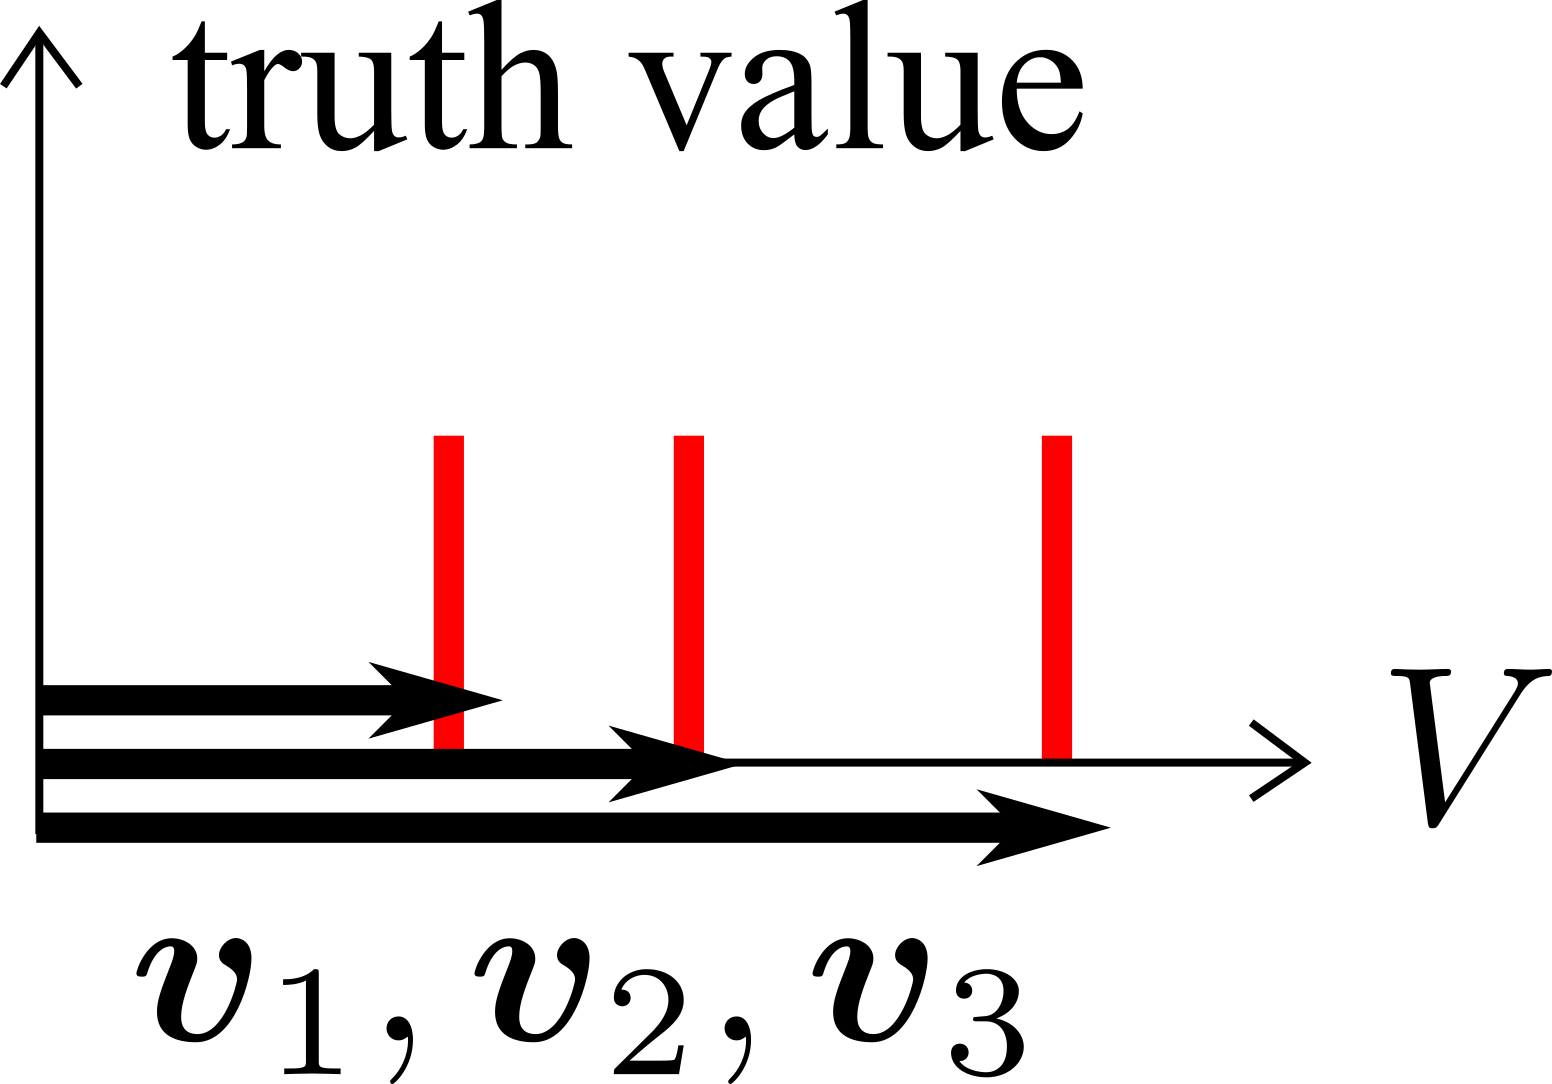
\includegraphics[scale=0.6]{Fourier-representation-0.png}}}
\quad \Rightarrow \quad
\vcenter{\hbox{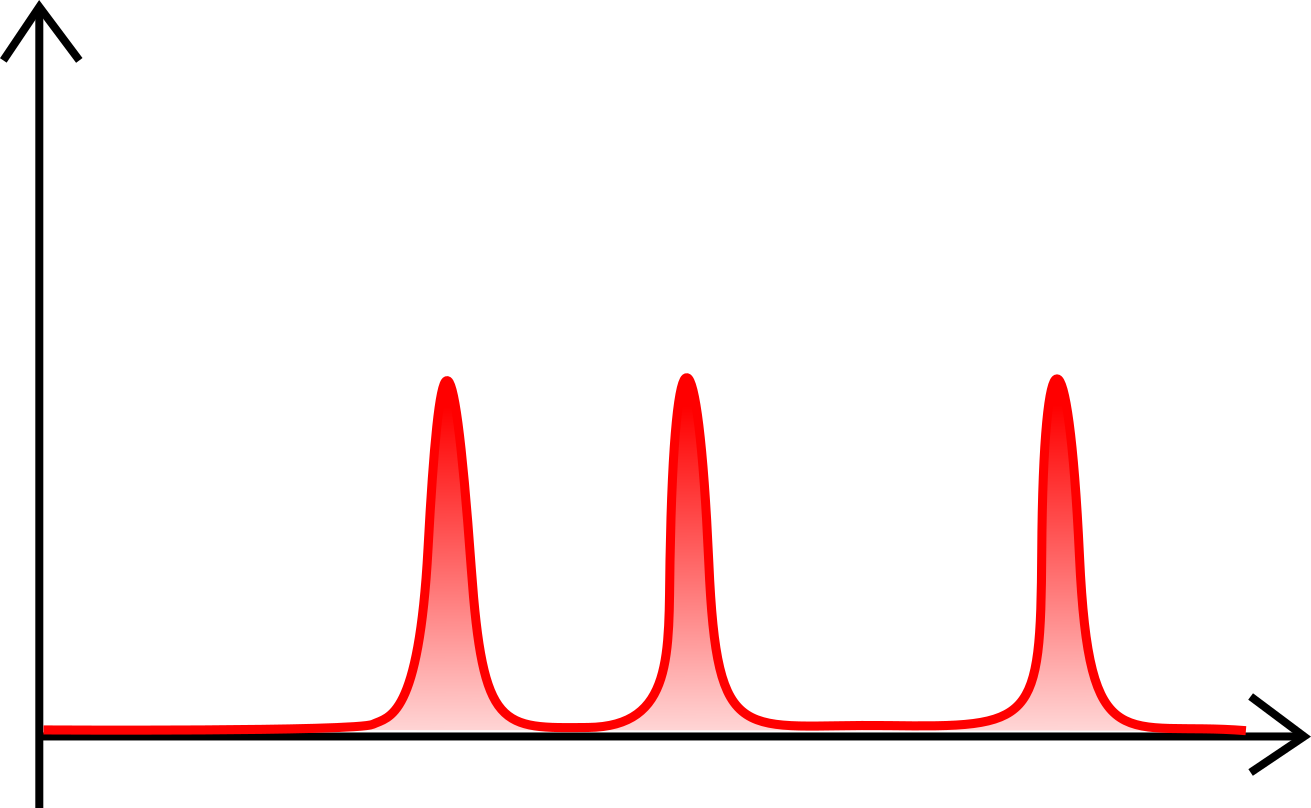
\includegraphics[scale=0.6]{Fourier-representation-0B.png}}}
\end{equation}

The resulting representation has some nice properties:
\begin{itemize}
	\item If we permute $(\vect{v}_1, \vect{v}_2, \vect{v}_3)$, the graph (and thus its spectrum) remains the same, \textit{ie}, the representation is \uline{invariant under permutations}
	\item We can add more vectors to the graph without changing the size of the spectral representation, \textit{ie}, it is relatively insensitive to the number of vectors
\end{itemize}

We can extend this idea to the \textbf{multi-dimensional} case where the literal proposition vector $\vect{p} \in \mathbb{P} = \mathbb{R}^{3d}$ 
\footnote{For example, a typical $d$ from Word2Vec or GloVe is 200, so $3d = 600$.}
and the state $\vect{x}$ consists of $k$ vectors $= \vect{p}_1 \wedge \vect{p}_2 \wedge ... \vect{p}_k$.  In other words, we need to apply Fourier transform to a wave over $3d$ dimensions.  Moreover, we can have truth values in the range $[-1,1]$, which can be construed as \textbf{fuzzy} truth values, or in the range $[0,1]$, regarded as the probability of \textbf{stochastic actions} (as is common in policy-gradient methods).
\begin{equation}
% \begin{tabular}{ccc}
% proposition vectors in $n$-dim space & & wave over $n$-dim space \\
% with {\color{red}truth values} \vspace*{0.5em} & & \\
\vcenter{\hbox{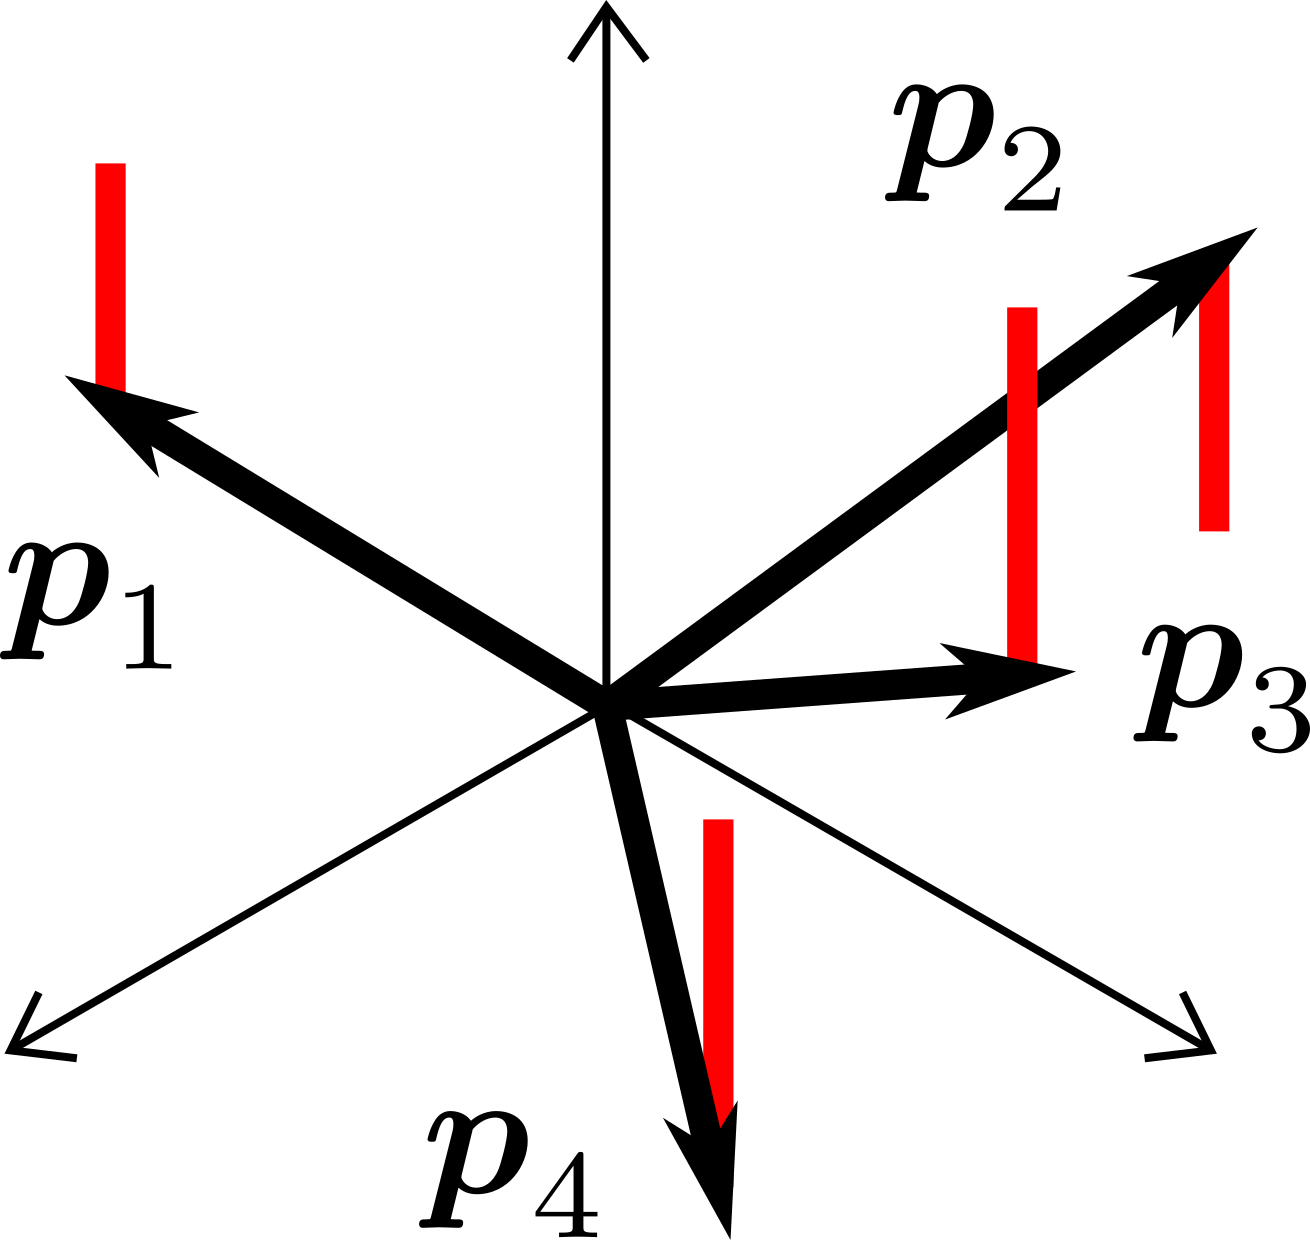
\includegraphics[scale=0.6]{Fourier-representation-1.png}}} 
\quad \Rightarrow \quad
\vcenter{\hbox{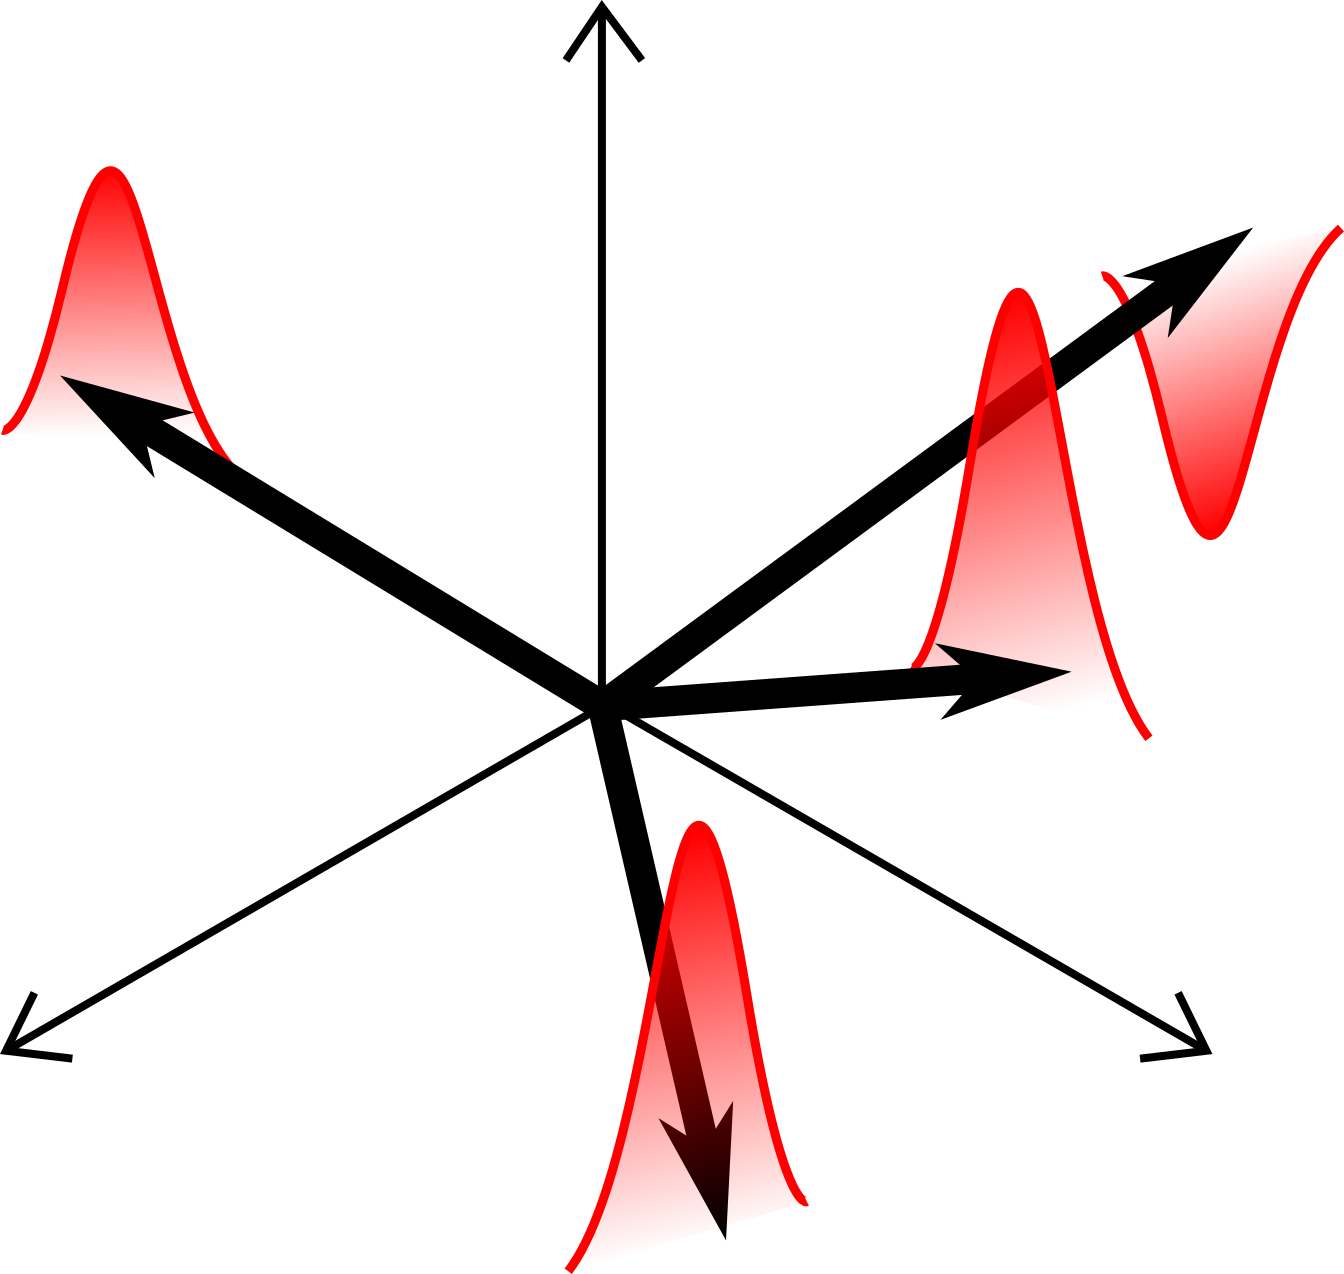
\includegraphics[scale=0.6]{Fourier-representation-2.png}}} 
% \end{tabular}
\end{equation}

Notice that our NN would \textit{input} from the spectral representation and \textit{output} the normal representation.

With this approach, the geometric shapes of (\ref{eqn:cylindric-shapes}) and (\ref{eqn:diagonal-shapes}) would be distorted in very complicated ways.  It remains to be verified whether NNs can learn this task effectively.

\section{PointNet's $g(h(x_1), ..., h(x_n))$ method}

\section{Conclusion}

This is unrelated to the paper's topic, but I would digress a bit into the area of AGI.

It seems that permutation invariance of neural networks is very difficult to achieve no matter which method we adopt.  So perhaps an alternative is to abandon the invariance entirely.

The idea is to use an attention mechanism to select a particular conjunction, to which the rule-applier performs the forward deduction step.  In this case, the conjunction can be a \textbf{sorted} concatenation of proposition vectors.  But this has the problem that the matcher and the rule-applier seems to be learning the same structures.

Assume that we have a conjunction that is ready for rule-application.  The possible patterns of deduction may be limited, and may be enumerable.  But we want to relax the ``rigid quantifications''.  

\printbibliography

\end{document}